\input{inc/estructura.tex}
\usepackage{amsmath}
\usepackage[nottoc,numbib]{tocbibind}
\usepackage{circuitikz}
\usepackage{tikz}
\usepackage{siunitx}
\usepackage{pgfplots}
\pgfplotsset{compat=1.18}
\usepgfplotslibrary{groupplots}
\usepackage{float}

\instituto{Universidad Tecnológica Nacional\\Facultad Regional Córdoba}
\carrera{Ingeniería Electrónica}
\title{Titulo}
\subtitledoc{Subtitulo}
\catedra{Catedra}
\professor{XXXXXXXXXX XXXXXXXX. \par XXXXXXXXXX XXXXXXXX.}
\curso{XRX}
\author{XXXXX XXXXX, XXXXX XXXXX. \par XXXXX XXXXX, XXXXX XXXXX.}
\legajo{XXXXX\par XXXXX}
\footerauthor{XXXXX, XXXXX}
\footerlegajo{XXXXX, XXXXX}
\footercatedra{XXXX}
\date{\today}

\begin{document} %Maximo 10 paginas
\maketitle
\tableofcontents
\newpage
\section{Introducción}
\section{Marco teorico}
\section{Primera Parte}
\subsection{Circuito}
\begin{center}
  \begin{circuitikz}[american]
    \draw (0,0) node[nujt, yscale=-1](ujt){}
    ;
    \draw (ujt.E) to[nos, mirror, invert, l=$L_2$] ++(-2,0)
    to[R] ++(-2,0)
    to[short] ++(0,1) node[vcc]{$V_{EE}$}
    ;
    \draw (ujt.B2) to[R] ++(0,2)
    to[nos, l=$L_1$] ++(0,1)
    to[short] ++(0,1) node[vcc]{$V_{CC}$}
    ;
    \draw (ujt.B1) to[short] ++(0,-1) node[ground];
  \end{circuitikz}
\end{center}
\subsection{Procedimiento}
\begin{enumerate}
  \item Armar el circuito seleccionando un correcto valor de las resistencias en
    función del datasheet del UJT.
  \item Abrir el interruptor L1 y cerrar el interruptor L2.
  \item Variar la $V_{EE}$ desde 0-30V y medir la corriente $I_E$.
  \item Completar la tabla propuesta modificándola si fuera necesario.
  \item Graficar la curva $I_E= f(V_{EE})$ con los datos relevados de la tabla.
  \item Abrir el interruptor L2 y cerrar el interruptor L1.
  \item Variar la VCC desde 0-30V y medir la corriente IB.
  \item Completar la tabla propuesta modificándola si fuera necesario.
\end{enumerate}
\subsection{Simulación}
\subsection{Experimental}
\begin{minipage}{0.2\linewidth}
\begin{tabular}{c|c|c}
  $V_{EE}$ &$V_{E}$ &$I_{E} [mA]$  \\
  \hline
  0   &0      &0       \\
  0.5 &0.52   &0.007   \\
  1   &0.79   &0.23    \\
  1.5 &0.88   &0.69    \\
  2   &0.94   &1.11    \\
  4   &1.03   &3.03    \\
  6   &1.06   &5.12    \\
  8   &1.09   &7       \\
  10  &1.12   &9.03    \\
  12  &1.15   &11.17   \\
  14  &1.17   &13.09   \\
  16  &1.20   &15.19   \\
  18  &1.22   &16.87   \\
  20  &1.24   &19.37   \\
  22  &1.26   &21.06   \\
  24  &1.28   &23.5    \\
  26  &1.30   &25.8    \\
  28  &1.32   &28.1    \\
  30  &1.34   &30
\end{tabular}
\end{minipage}
\begin{minipage}{0.8\linewidth}
\centering

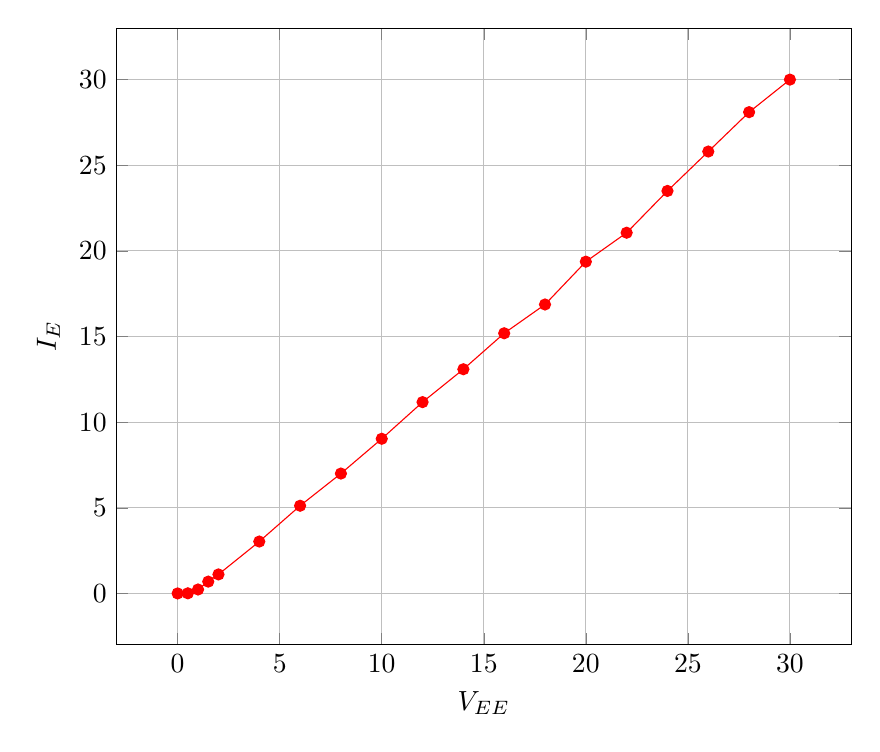
\begin{tikzpicture}
  \begin{axis}[
    width=.9\linewidth,
    xlabel = $V_{EE}$,
    ylabel = $I_{E}$,
    grid=major,
    ]
    \addplot[color=red,mark=*] coordinates {
      (0  , 0    )
      (0.5, 0.007)
      (1  , 0.23 )
      (1.5, 0.69 )
      (2 , 1.11 )
      (4 , 3.03 )
      (6 , 5.12 )
      (8 , 7    )
      (10, 9.03 )
      (12, 11.17)
      (14, 13.09)
      (16, 15.19)
      (18, 16.87)
      (20, 19.37)
      (22, 21.06)
      (24, 23.5 )
      (26, 25.8 )
      (28, 28.1 )
      (30, 30)
    };  
  \end{axis} 
\end{tikzpicture}

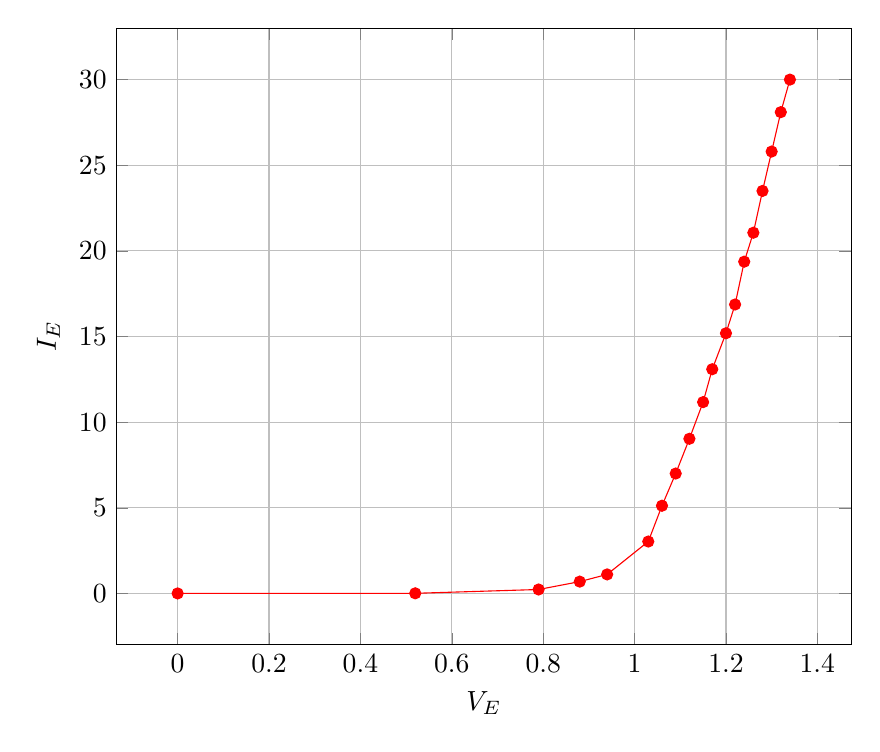
\begin{tikzpicture}
  \begin{axis}[
    width=.9\linewidth,
    xlabel = $V_{E}$,
    ylabel = $I_{E}$,
    grid=major,
    ]
    \addplot[color=red,mark=*] coordinates {
      (0    , 0    )
      (0.52 , 0.007)
      (0.79 , 0.23 )
      (0.88 , 0.69 )
      (0.94 , 1.11 )
      (1.03 , 3.03 )
      (1.06 , 5.12 )
      (1.09 , 7    )
      (1.12 , 9.03 )
      (1.15 , 11.17)
      (1.17 , 13.09)
      (1.20 , 15.19)
      (1.22 , 16.87)
      (1.24 , 19.37)
      (1.26 , 21.06)
      (1.28 , 23.5 )
      (1.30 , 25.8 )
      (1.32 , 28.1 )
      (1.34 , 30)
    };  
  \end{axis} 
\end{tikzpicture}

\end{minipage}

\begin{minipage}{0.2\linewidth}
\begin{tabular}{c|c|c}
  $V_{CC}$ &$V_{B_2}$ &$I_{B}$  \\
  \hline
  0   &0      &0    \\
  2   &1.71   &0.30 \\
  4   &3.57   &0.62 \\
  6   &5.23   &0.89 \\
  8   &6.96   &1.16 \\
  10  &8.90   &1.44 \\
  12  &10.69  &1.69 \\
  14  &12.37  &1.91 \\
  16  &14.27  &2.14 \\
  18  &16.29  &2.38 \\
  20  &17.82  &2.54 \\
  22  &19.67  &2.75 \\
  24  &22.2   &2.89 \\
  26  &23.8   &3.03 \\
  28  &25.6   &3.20 \\
  30  &27.4   &3.36 \\
\end{tabular}
\end{minipage}
\begin{minipage}{0.8\linewidth}
\centering
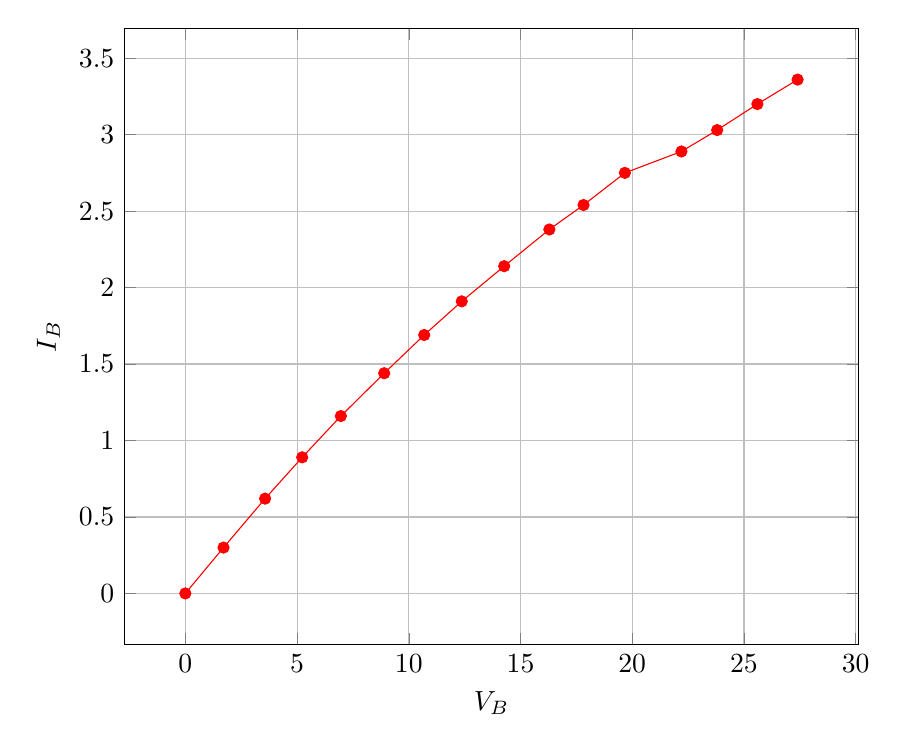
\begin{tikzpicture}
  \begin{axis}[
    width=.9\linewidth,
    xlabel = $V_{B}$,
    ylabel = $I_{B}$,
    grid=major,
    ]
    \addplot[color=red,mark=*] coordinates {
      (0     , 0    )
      (1.71  , 0.30 )
      (3.57  , 0.62 )
      (5.23  , 0.89 )
      (6.96  , 1.16 )
      (8.90  , 1.44 )
      (10.69 , 1.69 )
      (12.37 , 1.91 )
      (14.27 , 2.14 )
      (16.29 , 2.38 )
      (17.82 , 2.54 )
      (19.67 , 2.75 )
      (22.2  , 2.89 )
      (23.8  , 3.03 )
      (25.6  , 3.20 )
      (27.4  , 3.36 )
    };  
  \end{axis} 
\end{tikzpicture}
\end{minipage}
\begin{center}
 \begin{circuitikz}[american]
   \draw(0,0) to[R, l_=$r_{b2}$]++(0,3) to[short,-o]++(0,0) node[anchor=south](){$B_2$};
   \draw (0,0) to[vR, invert, l=$r_{b1}$]++(0,-3) to[short,-o]++(0,0) node[anchor=north](){$B_1$};
   \draw(-3,0) to[short,-o]++(0,0) node[anchor=east](){$E$} to[D](0,0)
 \end{circuitikz} 
\end{center}

\section{Segunda Parte}
\subsection{Circuito}
\begin{center}
  \begin{circuitikz}
    \draw (0,0) node[nujt, yscale=-1, xscale=-1](ujt){}
    ;
    \draw (ujt.B2) to[R, n=r1, l=100\unit{\ohm}] ++(0,2) coordinate(R100);
    \draw (ujt.B1) to[R, l=22\unit{\ohm}]++(0,-2) 
    to[short] ++(0,-0.5) node[ground]{}
    ;
  \draw (ujt.B2) to[short, -o]++(-1,0) node[anchor=east]{$OUT_1$};
  \draw (ujt.B1) to[short, -o]++(-1,0)node[anchor=east]{$OUT_2$};
  \draw (ujt.E) to[short,-*]++(2,0) coordinate(E) to[C, l=47nF]++(0,-2) node[ground]; 
  \draw (E) to[R, l=4.7K]++(0,2) to[pR, n=POT, l_=100k]++(0,2) coordinate(RPOT) to[short]++(0,1) node[vcc](VCC){$V_{CC}$};
  \draw (POT.wiper) to[short]++(-0.5,0) to[short]++(0,1) to[short, -*](POT|-RPOT);
  \draw (R100) to[short]++(0,1) node[vcc](){$V_{CC}$};
  \end{circuitikz}
\end{center}
\subsection{Procedimiento}
\begin{enumerate}
  \item Armar el circuito.
  \item Medir y graficar la señal en OUT1
  \item Medir y graficar la señal en OUT2
  \item Variar el potenciómetro y observar el efecto sobre la OUT1 y la OUT2 
\end{enumerate}
\subsection{Simulación}
\begin{center}
\begin{tikzpicture}
    \begin{groupplot}[
        group style={
            group size=1 by 4,
            x descriptions at=edge bottom,
            vertical sep=3pt,
        },
        width=0.95\linewidth,
        height=0.4\linewidth,
        grid=both,
        xlabel=$t$,
        thick
    ]
    \nextgroupplot[
      ylabel=$R_{POT}$,
      ]
        \addplot [red]  table [x index=0, y index=4]{./inc/sim/SegundaParte.txt};

    \nextgroupplot[
      ylabel=$V_{C}$,
      ytick={0,2,...,12}
      ]
        \addplot [blue]  table [x index=0, y index=3]{./inc/sim/SegundaParte.txt};
    \nextgroupplot[
      ylabel=$V_{B1}$,
      ytick={0,1,...,4}
      ]
        \addplot [teal]  table [x index=0, y index=1]{./inc/sim/SegundaParte.txt};
    \nextgroupplot[
      ylabel=$V_{B2}$,
      ]
        \addplot [violet]  table [x index=0, y index=2]{./inc/sim/SegundaParte.txt};
    \end{groupplot}
\end{tikzpicture}
\end{center}

\subsection{Experimental}

\section{Tercer Parte}
\begin{center}
  \begin{tabular}{l|c}
    Parametro &Valor \\ 
    \hline
    $\eta$          &  \\
    $R_{BBO}$       &  \\
    $V_{EB1(SAT)}$  &  \\
    $V_{(BR)B1E}$   &  \\
    $P_D$           &  \\
    $I_J$           &  
 \end{tabular} 
\end{center}

\section{Conclusión}
\end{document}
